\documentclass[../notes.tex]{subfiles}

\pagestyle{main}
\renewcommand{\chaptermark}[1]{\markboth{\chaptername\ \thechapter\ (#1)}{}}
\setcounter{chapter}{4}

\begin{document}




\chapter{Sequencing and Organelles}
\section{Sequencing and Next-Generation Sequencing}
\begin{itemize}
    \item \marginnote{10/25:}Yamuna wants us to call her by her first name.
    \item Spends the first 5 minutes glowing about teaching the class.
    \item As a postdoc, Yamuna worked at the bench next to the guys who developed Illumina sequencing.
    \item Sequencing represents the best of biochemistry because you have to know the chemistry to do it and the biology to interpret the results.
    \item Doing science via discovery (e.g., why is the sky blue?) vs. understanding (e.g., how does this work?).
    \begin{itemize}
        \item Chemical biology is the science of invention because you are trying to take the natural and control it.
    \end{itemize}
    \item What Yamuna wants us to take away: Understand how polymerases and everything works and then be able to tell what our sequence is.
    \begin{itemize}
        \item Sequencing is an exercise in tweaking the chemistry of biomolecules to get a certain result, enabled by the fact that we understand it so well.
    \end{itemize}
    \item DNA sequencing: Maxam-Gilbert, Sanger, Pyro (454) sequencing, Illumina, Nanopore, SMRT.
    \item Two principles that underlie DNA sequencing.
    \begin{itemize}
        \item Size-based separation on a gel (esp. for the older ones).
        \item \textbf{PCR}.
    \end{itemize}
    \item \textbf{Polymerase chain reaction}: A technique that amplifies (rapidly duplicates) a certain sequence of DNA millions or billions of times. \emph{Also known as} \textbf{PCR}.
    \begin{itemize}
        \item Suppose you have a strand of DNA and you want to know the sequence of a 150 bp bit.
        \item You need sufficient and sufficiently pure starting material to begin. Thus, if we have 50-100 copies of the DNA from extraction and mince them, the pieces will come out in different lengths.
        \item But we need way, way more copies to do meaningful chemistry and, moreover, we need only copies of the one specific set of base pairs.
        \item Solution: Polymerase chain reaction uses RNA polymerase, dNTPs, \ce{Mg^2+}, and some other things to make many many copies of just the 150 bps you're interested in.
        \item You need a primer (about 20-30 base pairs; what is necessary for specificity) that will sit on the beginning of the region.
        \item PCR uses a thermal cycler (a fancy oven that heats and cools between temperatures of your choosing at a rate of your choosing).
        \item DNA in an Eppendorf tube in the thermal cycler. We heat it to unwind the strands and then break the hydrogen bonding, yielding single-stranded DNA. Our forward and reverse primers sit on the single strands at the beginning of our target region. DNA polymerase attaches and copies until it falls off. Then we repeat.
        \item With every cycle, we increase/amplify the number of copies of target DNA vs. the variable length DNA. Thus, the variable length becomes more of an impurity. Now we can start to do chemistry.
        \item PCR was invented by Kary Mullis (who Yamuna isn't a fan of because he was a heavy user of LSD, downplayed humans' role in climate change, and doubted that HIV is the sole cause of AIDS).
        \item How do you create the primer if you haven't sequenced the DNA yet??
    \end{itemize}
    \item Separating DNA duplexes on the basis of size/length (\emph{not} polarity) using Agel (which is fancy TLC).
    \begin{itemize}
        \item If DNA is small, it will easily snake through the gel. If it is big, it will take longer.
        \item Like gel electrophoresis, you still have a cathode and anode. DNA (negatively charged due to phosphate groups) will move toward the cathode.
        \item Entirely pure substrate $\to$ one band.
        \item You can separate 48 bp strands from 49 bp strands.
        \item You have to chop up your DNA into reasonable sizes so that it can separate on a gel: 1000 vs. 1001? Not possible. 100 vs. 99? Possible. Resolution is better.
    \end{itemize}
    \item Huntington's genetic test.
    \begin{itemize}
        \item There is a protein/gene called Huntington. Everyone has a short number of repeats on the Huntington protein, but if you have two many (40+), you will develop Huntington's disease.
        \begin{itemize}
            \item 26-27 repeats is the border. This issue arises from polymerase "going nuts" and adding more repeats than it meant to.
            \item A \textbf{pathogenic} number of repeats vs. you being fine.
        \end{itemize}
        \item Amplify the section of your DNA containing the repeats. Then it is not necessary to sequence and count; you just need to determine the length of the repeating strand.
    \end{itemize}
    \item Cystic fibrosis.
    \begin{itemize}
        \item Often results from the $\Delta F508$ mutation (single AA mutation at phenylalanine 508).
        \item Yamuna's cousin died aged 36 from cystic fibrosis, but it wasn't $\Delta F508$ --- it was two "variant of unknown significance" mutations. Cases like hers allow us to canonize the noncanonical mutations.
    \end{itemize}
    \item 10 years, \$1 billion to sequence the entire human genome using Sanger sequencing (slow and very expensive).
    \begin{itemize}
        \item Someone else envisioned sequencing the entire human genome for \$1000 in a day.
        \item If feasible, it would have been great to understand all genomes, but instead, it helped us with COVID (detecting variants in a population and a person, virility, capacity for transmission).
        \item This saved many people by prevention (e.g., travel restrictions) before a cure (like the "mRNA vaccines") existed.
    \end{itemize}
    \item Back in 2005 when Yamuna started her lab in India, she would get data as a \textbf{sequence chromatogram}.
    \item \textbf{Seqeunce chromatogram}: A graph consisting of various colored peaks, each corresponding to one type of base pair.
    \begin{figure}[h!]
        \centering
        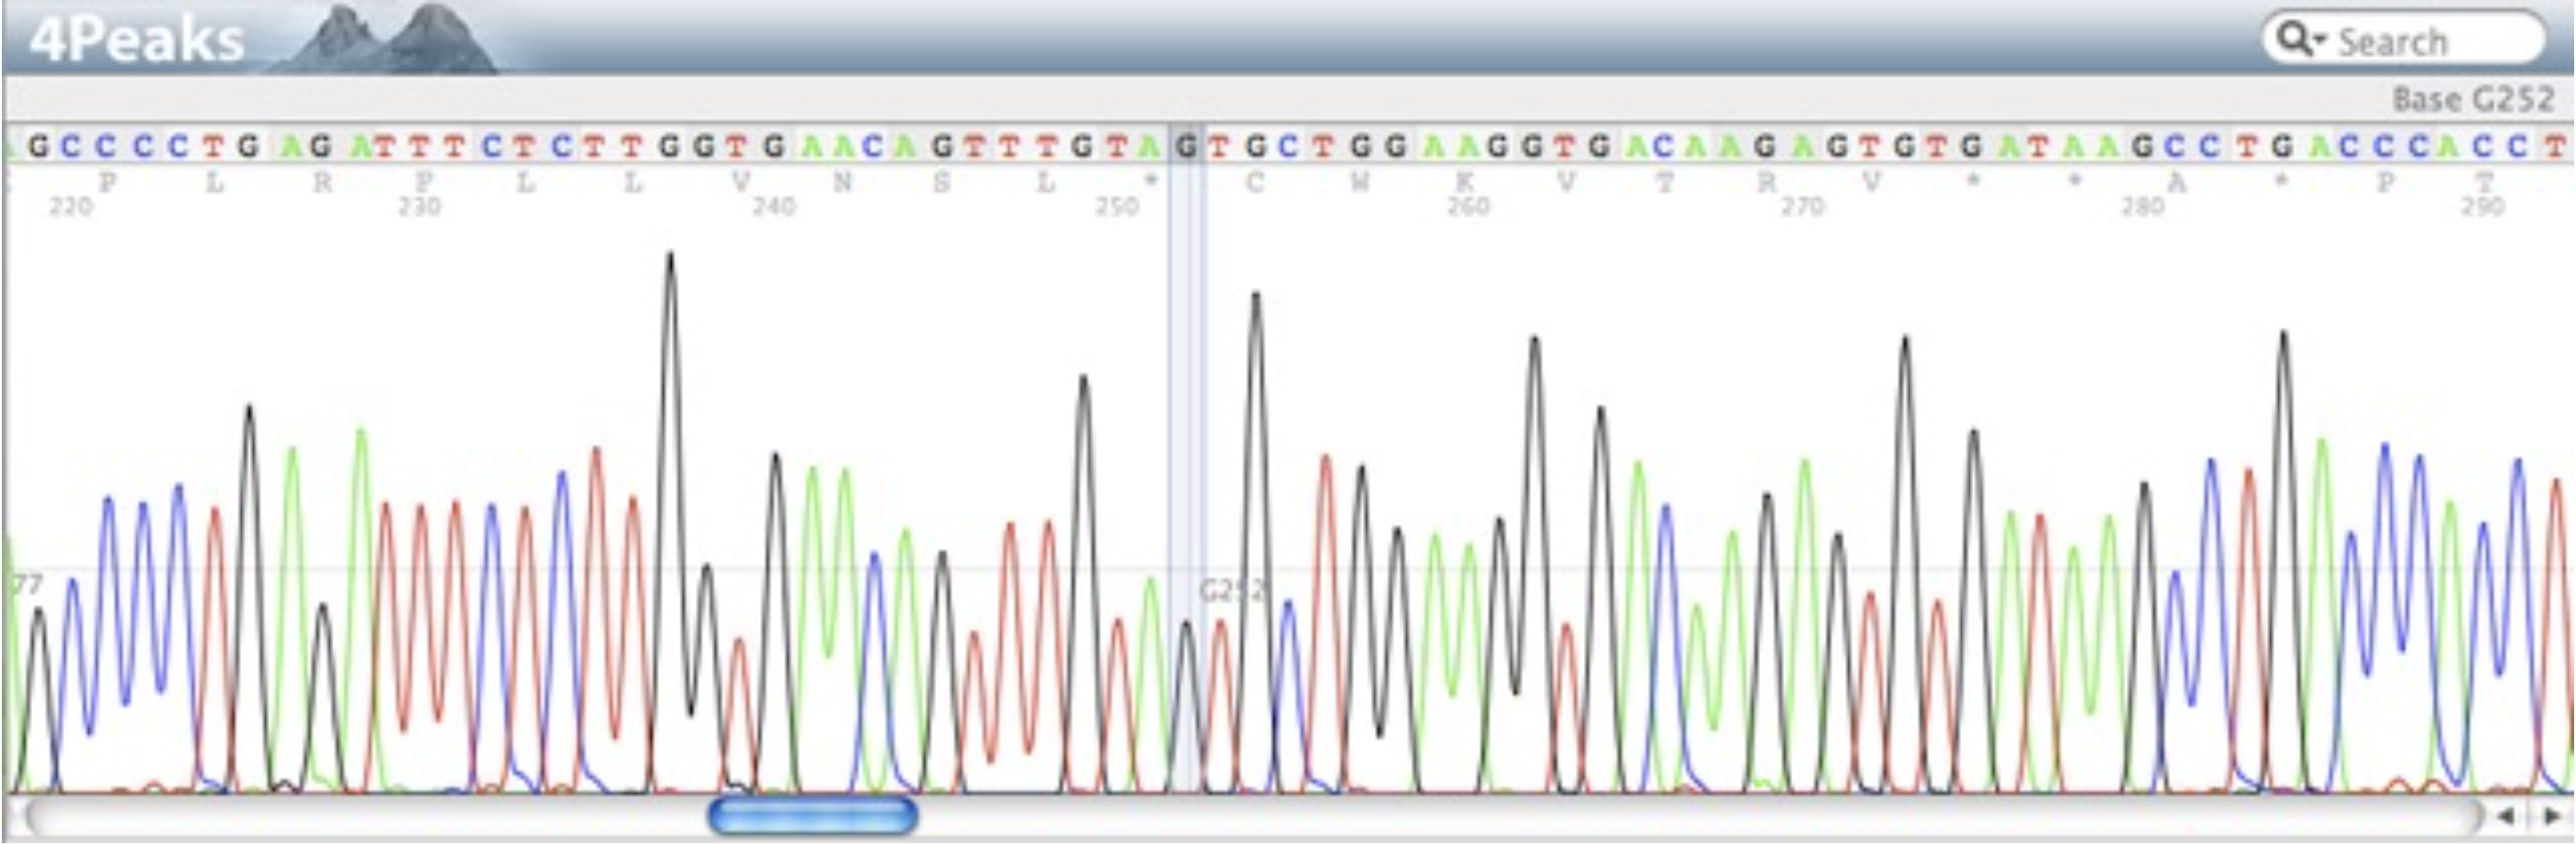
\includegraphics[width=0.7\linewidth]{../ExtFiles/sequenceChromatogram.png}
        \caption{Sequence chromatogram example.}
        \label{fig:sequenceChromatogram}
    \end{figure}
    \begin{itemize}
        \item Blue peak: Cytosine, Green peak: Adenine, Red peak: Thymine, Black peak: Guanine.
        \item Idiot-proofed for biologists to just read off their sequence from the top of the display window.
        \item How the graph is generated (briefly; this is Sanger sequencing).
        \begin{itemize}
            \item You write the sequence based on the length of the strand and how far it travels and which fluorescent dye has been attached to our gene.
            \item When DNA is being built, different dNTPs come in and sample the active site. If hydrogen bonding is correct, DNA polymerase locks into place, fuses it to the $3'$ end of the growing strand, and releases a \textbf{pyrophosphate}.
            \item This only happens when you have the right dNTP (there are energy barriers if you have the wrong one based on faulty hydrogen bonding).
            \item Release of a pyrophosphate is key to another sequencing method.
            \item Ability to make DNA artificially in a chemistry lab (Caruthers, 1985). You can attach literally anything to the growing $3'$ end. This allows you to create primers that set an address.
            \begin{itemize}
                \item Yamuna believes this should have won a Nobel prize since it's been the basis for several others.
            \end{itemize}
            \item If you attach a ddNTP to the growing end, you stop growth.
        \end{itemize}
    \end{itemize}
    \item \textbf{Pyrophosphate}: Two phosphates bound via a single linking oxygen, i.e., \ce{P2O7^4-}. \emph{Denoted by} \textbf{PPi}.
    \item Maxam-Gilbert sequencing.
    \begin{itemize}
        \item Developed by Wally Gilbert and Allan Maxam.
        \begin{itemize}
            \item Gilbert and Sanger originally won the Nobel Prize for sequencing.
        \end{itemize}
        \item Know this for historical reasons; came out second, but was adopted first.
        \item Start with a bunch of copies (circa 1 million) of a DNA strand obtained using bacterial cloning.
        \item Label the $5'$ end of each sequence with \ce{{}^32P}.
        \item Divvy up the labeled DNA between four Eppendorfs. To each tube, add a chemical that is selective for one or two nucleobases. Add just enough of the chemical so that every strand will react once. Remember that most strands will not react. Then introduce hot piperidine (Yamuna said hydrazine??) to cleave the strand right before (Yamuna says after??) the modification.
        \item Chemicals:
        \begin{align*}
            \text{A}+\text{g} &= \ce{HCOOH}&
            \text{G} &= \ce{Me2SO4}&
            \text{T}+\text{c} &= \ce{N2H4}&
            \text{C} &= \ce{N2H4 + NaCl}
        \end{align*}
        \item Running these mixtures on a gel will lead to bands corresponding to each cut and unreacted strands.
        \item The strand that travels the farthest (is the lightest/shortest) corresponds to the first nucleobase. The strands that travel the least are the unreacted strands.
        \begin{itemize}
            \item Example 1: No band in the $\text{T}+\text{c}$ column and a band in the $\text{C}$ columns? Cytosine.
            \item Example 2: Bands at the same level in the $\text{A}+\text{g}$ and $\text{G}$ columns? Guanine.
        \end{itemize}
    \end{itemize}
    \item Sanger sequencing.
    \begin{itemize}
        \item When cloning became pass\'{e}, everyone switched to Sanger.
        \item Two methods of Sanger sequencing: Sequential and parallel.
        \item Sequential Sanger sequencing.
        \begin{itemize}
            \item Amplify your region of interest using PCR.
            \item However, during this process, add a small amount (1-5\%) of a specific dideoxynucleotide (ddNTP). If you include a small amount of ddATP for example, then whenever DNA polymerase matches one of these with a thymine and incorporates it into the growing strand, the strand will not be able to grow any further (there is no longer a $3'$ hydroxyl to bond the next nucleotide to).
            \item This will allow you to generate stops at every nucleobase of a certain type.
            \item Doing this for every nucleobase independently and then running all four samples on a gel gives you a similar result to Maxam-Gilbert sequencing, except that this time, our result is analogous to cleaving after the "modification" and we don't have "leaks" as with the $\text{T}+\text{c}$ and $\text{A}+\text{g}$ chemicals.
        \end{itemize}
        \item Parallel Sanger sequencing.
        \begin{itemize}
            \item Amplify your region of interest using PCR.
            \item However, during this process, add a small amount (1-5\%) of fluorophore-labeled ddNTPs such that each of the four ddNTPs fluoresces a different color. Incorporating these will guarantee that each strand of DNA ends in a fluorophore-labeled ddNTP.
            \item These strands can be separated with high accuracy using capillary gel electrophoresis.
            \begin{itemize}
                \item Capillary gel electrophoresis is very fancy gel --- very long and very thin.
            \end{itemize}
            \item As each strand moves through the capillary, it eventually passes by a light fluorescence detector.
            \item This generates the sequence chromatogram.
        \end{itemize}
        \item Better since it doesn't have radioactivity, once fluorophores became stable, and after the advent of capillary gel electrophoresis.
    \end{itemize}
    \item Svante P\"{a}\"{a}bo at the Max Planck Institute won the 2022 Nobel Prize in Physiology or Medicine for sequencing the Neanderthal genome.
    \begin{itemize}
        \item He extracted DNA from skulls and bones. Every bit of DNA was missing something, but by sequencing enough and comparing, he was able to fully reconstruct it.
        \item He did this with \textbf{pyrosequencing}, which many biologists had forgotten about.
    \end{itemize}
    \item \textbf{Pyrosequencing}: A sequencing by synthesis method that works as follows. \emph{Also known as} \textbf{454 sequencing}. \emph{Procedure}
    \begin{enumerate}
        \item Begin with a pure set of DNA sequences generated via PCR. Bind adapters to the sequences, and biotin to the adapters. Immobilize multiple copies of the sequence each of a number of streptavidin beads.
        \item Bind a primer to each sequence and attach DNA polymerase.
        \item Add a specific dNTP (dATP, dTTP, dGTP, or dCTP).
        \item Suppose the first base to be sequenced/synthesized is adenine and dATP is the first dNTP added. Then DNA polymerase will click dATP into place, releasing a pyrophosphate.
        \item The PPi is used by ATP-sulfurylase to generate a molecule of ATP.
        \item This allows Luciferase to use ATP and its substrate to generate a flash of light.
        \item Before adding in another type of dNTP, it is necessary to remove the previous one. This is accomplished by adding apyrase, an enzyme that converts all available dNTPs to dNDPs and then inactive dNMPs.
        \item Counting the number of flashes of light after a dNTP is produced tells us how many of that dNTP in a row there are at that point.
    \end{enumerate}
    \item Example of pyrosequencing.
    \begin{itemize}
        \item Consider the strand ATGGCCC.
        \item Introducing dATP, dGTP, or dCTP at first will lead to no flashes of light. Introducing dTTP will lead to one flash of light (because T binds with A and there is one A).
        \item Similarly, introducing anything other than dATP next will lead to nothing, and introducing dATP will lead to one flash of light.
        \item Now introducing dCTP will lead to two consecutive flashes of light (as two pyrophosphates are released from the addition of two dCTPs to the growing strand, one for each dGTP in the guiding strand).
        \item Lastly, introducing dGTP will lead to three consecutive flashes of light. 
    \end{itemize}
    \item Notes on pyrosequencing.
    \begin{itemize}
        \item 454 is what the company referred to the technology as before it was released and named "pyrosequencing."
        \item Pyrosequencing is the bridge between the ways Yamuna used as a grad student and what we do today.
        \item In an analogy, ATP-sulfurylase is like the light switch, luciferase is like the lightbulb, and apyrase is like the eraser between steps.
        \item You generate a bead with many copies of a specific strand on it.
        \item How this works in a system:
        \item Take DNA, sonicate it to break it up, make the library, add adapters.
        \item Emulsion PCR (little droplets of water in a mix of oil that contain dNTPs, primers, water, polymerase, etc.).
        \item Relation to chemistry 1-bead, 1-compound question.
        \item Strand that is not covalently bonded comes back and reattaches.
        \item PCR amplification occurs until every strand displays the same DNA sequencing.
        \item Many wells; each one contains a single DNA sequence. Then flow in dATP plus an enzyme cocktail.
        \item You need a big flash of light (multiple photons --- 20-30 flashing at the same time).
        \item Your computer flows in different bases to different wells and seeing what gives you a flash.
        \item Allows you to sequence in a massively parallel way.
    \end{itemize}
    \item Illumina sequencing (currently the most important method).
    \begin{itemize}
        \item Sequences 200-300 bps at a time.
        \item Nanopore and SMRT sequencing give you extremely long sequences, but most big biological discoveries today are based on Illumina sequencing.
        \item Once you have your sequences of interest, you attach primers and...
        \item Attach your strands to the surface of a wafer.
        \item Bridge synthesis on the wafer.
        \item You get a flash of light whenever you add.
        \item You get an answer from your entire surface instead of just a single molecule. Since DNA polymerase makes errors, this eliminates them via the law of averages.
        \item The cost of sequencing is now in storing the data, not in the reagents.
        \item Five major challenges to solve to achieve next generation sequencing (NGS) by Illumina.
        \begin{itemize}
            \item The $3'$ OH problem.
            \begin{itemize}
                \item If you want to protect the $3'$ OH with a fluorophore, you have a 2 hour deprotonation. This means that it will take 25 days to sequence 300 bases.
                \item If you use 2-o-nitrophenol, you have a UV-deprotonation. Instaneous but skin cancer.
                \item Single color readout is impractical; thus, you need a four-color readout.
                \item The ideal $3'$ OH protecting group is small, stable under aqueous conditions, has quantitative cleavage and high turnover, and preserves the DNA integrity.
            \end{itemize}
            \item The fluorophore problem.
            \item The polymerase problem.
            \item The surface chemistry problem.
            \item The problem of polymerase-generated errors and parallelization.
        \end{itemize}
    \end{itemize}
    \item Check out videos online.
\end{itemize}




\end{document}